\section{Workflow}

Le workflow Galaxy fournit un ensemble d’outils pour la manipulation et l’analyse de données génomiques. Il est très intuitif dans l’utilisation ce qui en fait une cible de choix pour le biologiste.\\


Il permet de créer des workflows, les enregistrer dans un espace dédié, les partager, et les exécuter de façon automatique. Les outils dédiés analyse de données NGS sont régulièrement mis à jour.\\


Galaxy offre donc la possibilité d’exécuter des analyses bioinformatiques sans effort de programmation. La version en ligne est intéressante car elle permet de se familiariser aux logiciels et d'exécuter l’analyse depuis un portable, mais la possibilité d’intégrer ces propres outils est indéniablement un gros avantage de la version locale.\\

Si nous devions citer un inconvénient, plutôt d’actualité : l’utilisateur est obligé de charger ses données en mémoire dans Galaxy, le temps de chargement peut être très long si l’on manipule des données issues d’expériences NGS, même sur une instance locale. Il est impensable de charger de telles données sur la version web.\\

Prenons par exemple un workflow de métagénomique (Fig. 18).\\

\begin{figure}[!h]
 \centering
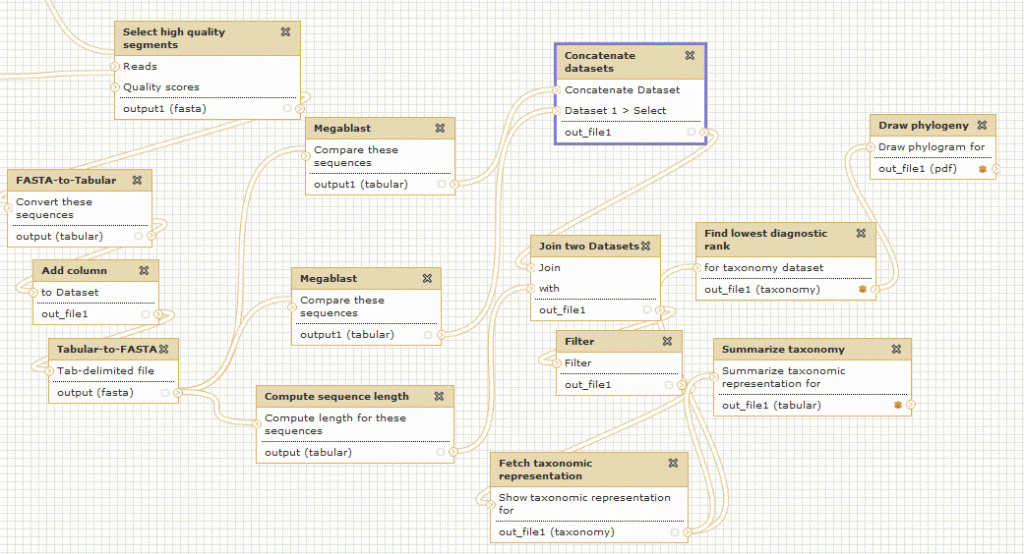
\includegraphics[scale=0.4]{Images/metagenomics.png}
\caption{Workflow de métagénomique.}
\end{figure}

La métagénomique étudie les organismes microbiens directement dans leur environnement sans passer par une étape de culture en laboratoire. Dans ce cas nous cherchons à obtenir des informations relatives à l'origine phylogénétique de l'organisme étudié et aussi des informations taxonomiques.\\
Pour cela, le workflow prend en entrée des fichiers issu de NGS 454. Dans la première entrée le workflow demande le fichier de read et la deuxième entrée celui de qualité.
\newpage

Ensuite, ces données passe par un programme chargé de sélectionner les segments de plus grande qualité. Ce programme à comme sortie un fichier au format FASTA.  Le principe ensuite est de lancer deux mégaBlast pour comparer les séquences à deux bases de données différentes. Mais pour cela il faut que chaque séquence "de qualité" soit identifiée donc on passe le fichir FASTA sortant du premier programme dans un convertisseur vers un format tabular, on rajoute une colonne qui content le numéro du read et on repasse au format FASTA.\\
 
En parallèle on lance un programme qui retourne un tableau avec dans la première colonne le nom de la séquence et dans la deuxième la longueur en acide nucléique. Les sorties des fichiers de blast sont mises dans un même fichier. Le tableau de longueur des séquences est lui aussi agrégé dans un autre programme. Le fichier sortant de ce programme passe dans un nouveau programme qui lui prépare les informations pour l'analyse taxonomique et l'analyse phylogénétique.\\

Donc la sortie de ce programme est envoyée à deux autres programmes un pour l'analyse phylogénétique et l'autre pour la finalisation de l'analyse taxonomique. Au final on obtient un fichier au format PDF avec l'arbre phylogénétique et un fichier comportant toute les informations taxonomiques.\\



Ce qui est agréable dans un tel type de workflow est la simplicité de mise en place, surtout avec l'interface graphique ou les programme sont représenté par des boites relié entre elles part des flèches. Ces flèches correspondent aux fichiers qui vont d'une application à un autre.\\